\usepackage{booktabs}
\usepackage{longtable}
\usepackage{array}
\usepackage{multirow}
\usepackage{wrapfig}
\usepackage{float}
\usepackage{colortbl}
\usepackage{pdflscape}
\usepackage{tabu}
\usepackage{threeparttable}
\usepackage{threeparttablex}
\usepackage[normalem]{ulem}
\usepackage{makecell}
\usepackage{xcolor}

% % set background image if you will
% \usebackgroundtemplate%
% {%
%     \includegraphics[width=\paperwidth,height=\paperheight]{02-dna_modification_background_dna_helix.jpg}%
% }

% % set background in a TikZ node for modifications
% % set background in a TikZ node for modifications
\usepackage{tikz}
\usepackage[absolute,overlay]{textpos}
\setbeamertemplate{title page}{
\tikz\node[opacity=0.9] {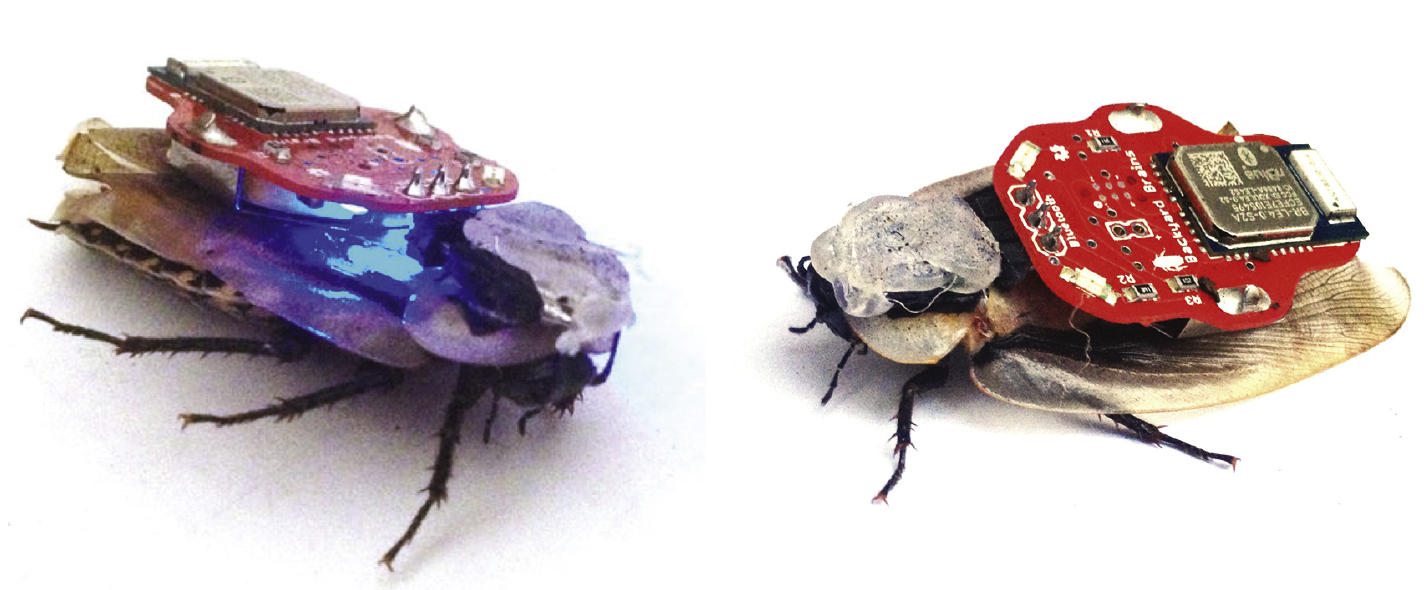
\includegraphics[width=0.8\paperwidth]{./07-bioethics_cover.png}};
% \tikz\node[opacity=0.8] {\includegraphics[width=5cm,ext=.1-overview_mutation_cover.png,type=png,read=.1-overview_mutation_cover.png]{1}} % if name shall contain dots, suppose filename = 01.1-overview_mutation_cover.png
\begin{textblock}{20}(1.5,2.8)\usebeamerfont{title} % 1.5 is x position in page
{\color{blue}\raggedright\par\inserttitle}
\end{textblock}
\begin{textblock}{7.5}(1.5,7) % 1.5 is x position in page
{\color{gray}\raggedright{\insertauthor}\mbox{}\\[0.2cm]
\insertdate}
\end{textblock}} % dd_rookie modified, figure is top aligned

% % set caption font size
% % note that beamer presentation native captions have their own configs
% \usepackage{caption}
% \captionsetup{font=footnotesize}

% this font option is amenable for beamer
\setbeamerfont{caption}{size=\tiny}

% some beamer themes naturally might not support navigation symbols
% \setbeamertemplate{navigation symbols}{} % remove navigation symbols

\setbeamertemplate{footline}[page number] % insert page number in footline

% \setbeamertemplate{navigation symbols}{slide} % insert slide indication in navigation
% \setbeamertemplate{navigation symbols}{frame} % insert frame indication in navigation
% \setbeamertemplate{navigation symbols}{section} % insert section indication in navigation
% \setbeamertemplate{navigation symbols}{subsection} % insert subsection indication in navigation

% \AtBeginSubsection{} % supress subsection display
